\documentclass{beamer}

\usepackage{amsfonts}
\usepackage{listings}
\usepackage{adjustbox}
\usepackage{tikz}
\usetikzlibrary{chains,arrows,automata,decorations.markings,positioning,calc,decorations.pathreplacing,patterns}

\setbeamertemplate{footline}[frame number]

\begin{document}

\frame{
    \begin{center}
        \textbf{\huge Vector instructions}

        Wojciech Muła, \href{http://0x80.pl}{0x80.pl} January 2021

        {\small Thanks to Roman Kurc for valuable feedback}
    \end{center}

    \vfill

    \pause
    What do we cover?

    \begin{itemize}
        \pause
        \item What are \textbf{vector instructions}/\textbf{SIMD instructions}
        \pause
        \item Why are they important
        \pause
        \item How do they work
        \pause
        \item What are good for
    \end{itemize}

    \vfill
}

\frame{
    \frametitle{Where can we find vectors?}

    \begin{itemize}
        \pause
        \item Shortly: vectors are \emph{everywhere}
        \pause
        \item All kinds of engineering simulations (mechanical, electrical, chemical)
        \pause
        \item Scientific simulations (weather forecasting, detecting black holes, looking for new particles)
        \pause
        \item Digital signal processing (sound, video, 3D graphics, computer vision, compression)
        \pause
        \item Machine Learning\pause\ (sorry for the buzzword)
    \end{itemize}
}

\frame{
    \frametitle{What is a vector?}

    \begin{itemize}
        \item In maths a \textbf{vector} is a sequence of numbers (\emph{scalars})
        \pause
        \item The IT world uses the term \textbf{array} for vectors
        \pause
        \item In programming an array of numbers models a vector\\
              $v = (1, 2, 3)$ $\Rightarrow$ \texttt{int v[3] = \{1, 2, 3\};} {\tiny (C/C++/Java)}
              $v = (1, 2, 3)$ $\Rightarrow$ \texttt{v = [1, 2, 3]} {\tiny (Python)}
        \pause
        \item An array can hold anything, not only bare numbers, but
              also pixels (images), samples (sound), points (3D models),
              characters (text)
    \end{itemize}
}

\frame{
    \frametitle{How would we add two vectors? -- part 1}

    Suppose we have two vectors of size 8:

    \pause
    $$a = (1, 2, 3, 4, 5, 6, 7, 8)$$

    \pause
    $$b = (7, 1, 4, 2, 3, 5, 1, 0)$$

    \pause
    Their sum $c$ is:

    $$c = a + b = (8, 3, 7, 6, 8, 11, 8, 8)$$
}

\frame{
    \frametitle{How would we add two vectors? -- part 3}

    A program that performs vector addition is quite simple:
    \lstinputlisting[language=C++]{vector-add-naive.cpp}

    \pause
    It can be written with a loop:
    \lstinputlisting[language=C++]{vector-add-loop.cpp}
}

\frame{
    \frametitle{How would we add two vectors? -- part 4}

    \lstinputlisting[language=C++]{vector-add-loop.cpp}

    \vfill

    \pause
    Despite the form, the number of basic instruction is:

    \begin{itemize}
        \pause
        \item 16 loads from memory (\texttt{a[0..7]} and \texttt{b[0..7]})
        \pause
        \item 8 additions (\texttt{+})
        \pause
        \item 8 stores to memory (\texttt{c[0..7]})
    \end{itemize}

    \vfill
}

\frame{
    \frametitle{Hardware dedicated to vector operations}

    \begin{itemize}
        \pause
        \item CPUs can boost vector operations by providing dedicated \textbf{vector instructions}
        \pause
        \item \ldots often called \textbf{SIMD} instructions
        \pause
        \item A vector instruction is a hardware implementation of given basic vector operation
        \pause
        \item Vector instructions were provided by supercomputers even in 1960's
        \pause
        \item In commodity hardware used in PC, laptops, phones the first vector instructions
              appeared in late 1990's
        \pause
        \item GPUs usually have vector execution units
    \end{itemize}
}

\frame{
    \frametitle{What is SIMD?}

    \begin{itemize}
        \pause
        \item James Flynn in 1970's introduced rough classification of \emph{computer systems}
        \pause
        \item A computer can have \textbf{single} or \textbf{multiple} CPUs
        \pause
        \item \ldots thus can execute single/multiple instructions at once
        \pause
        \item An instruction can deal with either \textbf{single} or \textbf{multiple} data at once
        \pause
        \item SIMD means: \emph{Single Instructions, Multiple Data}
        \pause
        \item Here "multiple data" means "a vector"
        \pause
        \item Most \textbf{CPU cores} work in SISD model: \emph{Single Instruction, Single Data}
    \end{itemize}
}

\frame{
    \frametitle{How vector instructions work? --- part 1}

    Suppose vectors have 8 elements

    Operation is $c = a + b$

    \begin{center}
        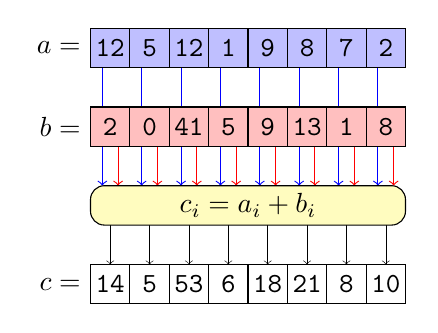
\begin{tikzpicture}
\draw[->,color=blue] (3.650,0.000) -- (3.650,-1.500);
\draw[->,color=red] (3.850,-1.000) -- (3.850,-1.500);
\draw[very thin,->] (3.750,-1.750) -- (3.750,-2.500);
\draw[->,color=blue] (3.150,0.000) -- (3.150,-1.500);
\draw[->,color=red] (3.350,-1.000) -- (3.350,-1.500);
\draw[very thin,->] (3.250,-1.750) -- (3.250,-2.500);
\draw[->,color=blue] (2.650,0.000) -- (2.650,-1.500);
\draw[->,color=red] (2.850,-1.000) -- (2.850,-1.500);
\draw[very thin,->] (2.750,-1.750) -- (2.750,-2.500);
\draw[->,color=blue] (2.150,0.000) -- (2.150,-1.500);
\draw[->,color=red] (2.350,-1.000) -- (2.350,-1.500);
\draw[very thin,->] (2.250,-1.750) -- (2.250,-2.500);
\draw[->,color=blue] (1.650,0.000) -- (1.650,-1.500);
\draw[->,color=red] (1.850,-1.000) -- (1.850,-1.500);
\draw[very thin,->] (1.750,-1.750) -- (1.750,-2.500);
\draw[->,color=blue] (1.150,0.000) -- (1.150,-1.500);
\draw[->,color=red] (1.350,-1.000) -- (1.350,-1.500);
\draw[very thin,->] (1.250,-1.750) -- (1.250,-2.500);
\draw[->,color=blue] (0.650,0.000) -- (0.650,-1.500);
\draw[->,color=red] (0.850,-1.000) -- (0.850,-1.500);
\draw[very thin,->] (0.750,-1.750) -- (0.750,-2.500);
\draw[->,color=blue] (0.150,0.000) -- (0.150,-1.500);
\draw[->,color=red] (0.350,-1.000) -- (0.350,-1.500);
\draw[very thin,->] (0.250,-1.750) -- (0.250,-2.500);
\draw [fill=yellow!25,rounded corners=5pt] (0.000,-2.000) rectangle (4.000,-1.500);
\node[] at (2.000,-1.750) {$c_i = a_i + b_i$};
\node[anchor=east] at (0.000,0.250) {$a=$};
\node[anchor=east] at (0.000,-0.750) {$b=$};
\node[anchor=east] at (0.000,-2.750) {$c=$};
\draw [fill=blue!25] (3.50, 0.00) rectangle (4.00, 0.50);
\node at (3.75, 0.25) {\texttt{2}};
\draw [fill=blue!25] (3.00, 0.00) rectangle (3.50, 0.50);
\node at (3.25, 0.25) {\texttt{7}};
\draw [fill=blue!25] (2.50, 0.00) rectangle (3.00, 0.50);
\node at (2.75, 0.25) {\texttt{8}};
\draw [fill=blue!25] (2.00, 0.00) rectangle (2.50, 0.50);
\node at (2.25, 0.25) {\texttt{9}};
\draw [fill=blue!25] (1.50, 0.00) rectangle (2.00, 0.50);
\node at (1.75, 0.25) {\texttt{1}};
\draw [fill=blue!25] (1.00, 0.00) rectangle (1.50, 0.50);
\node at (1.25, 0.25) {\texttt{12}};
\draw [fill=blue!25] (0.50, 0.00) rectangle (1.00, 0.50);
\node at (0.75, 0.25) {\texttt{5}};
\draw [fill=blue!25] (0.00, 0.00) rectangle (0.50, 0.50);
\node at (0.25, 0.25) {\texttt{12}};
\draw [fill=red!25] (3.50, -1.00) rectangle (4.00, -0.50);
\node at (3.75, -0.75) {\texttt{8}};
\draw [fill=red!25] (3.00, -1.00) rectangle (3.50, -0.50);
\node at (3.25, -0.75) {\texttt{1}};
\draw [fill=red!25] (2.50, -1.00) rectangle (3.00, -0.50);
\node at (2.75, -0.75) {\texttt{13}};
\draw [fill=red!25] (2.00, -1.00) rectangle (2.50, -0.50);
\node at (2.25, -0.75) {\texttt{9}};
\draw [fill=red!25] (1.50, -1.00) rectangle (2.00, -0.50);
\node at (1.75, -0.75) {\texttt{5}};
\draw [fill=red!25] (1.00, -1.00) rectangle (1.50, -0.50);
\node at (1.25, -0.75) {\texttt{41}};
\draw [fill=red!25] (0.50, -1.00) rectangle (1.00, -0.50);
\node at (0.75, -0.75) {\texttt{0}};
\draw [fill=red!25] (0.00, -1.00) rectangle (0.50, -0.50);
\node at (0.25, -0.75) {\texttt{2}};
\draw [] (3.50, -3.00) rectangle (4.00, -2.50);
\node at (3.75, -2.75) {\texttt{10}};
\draw [] (3.00, -3.00) rectangle (3.50, -2.50);
\node at (3.25, -2.75) {\texttt{8}};
\draw [] (2.50, -3.00) rectangle (3.00, -2.50);
\node at (2.75, -2.75) {\texttt{21}};
\draw [] (2.00, -3.00) rectangle (2.50, -2.50);
\node at (2.25, -2.75) {\texttt{18}};
\draw [] (1.50, -3.00) rectangle (2.00, -2.50);
\node at (1.75, -2.75) {\texttt{6}};
\draw [] (1.00, -3.00) rectangle (1.50, -2.50);
\node at (1.25, -2.75) {\texttt{53}};
\draw [] (0.50, -3.00) rectangle (1.00, -2.50);
\node at (0.75, -2.75) {\texttt{5}};
\draw [] (0.00, -3.00) rectangle (0.50, -2.50);
\node at (0.25, -2.75) {\texttt{14}};
\end{tikzpicture}

    \end{center}
}

\frame{
    \frametitle{How vector instructions work? --- part 2}

    How it looks like in code:
    \pause
    \vfill
    \begin{adjustbox}{max width=10cm}
        \lstinputlisting[language=C++]{vector-add-hardware.cpp}
    \end{adjustbox}

    \vfill

    \begin{itemize}
        \pause
        \item In traditional approach we had 32 instructions

        \pause
        \item \texttt{vector\_foo} represents a \textbf{single CPU instruction}

        \pause
        \item Only four instructions are executed in total

        \pause
        \item Both approaches perform exactly the same program: the same
              amount of data is transferred from/to memory, the same number
              of additions is executed
    \end{itemize}

    \vfill
}

\frame{
    \frametitle{Is SIMD really faster?}

    \begin{itemize}
        \pause
        \item "a vector instruction" doesn't just  mean "a hardware loop"
        \pause
        \item vector instructions do have dedicated execution units
        \pause
        \item \ldots which perform elementary operations \textbf{in parallel}
        \pause
        \item for example on Intel Skylake-X:
        \pause
        \item \ldots addition of two 8-bit numbers takes\pause\relax~1 CPU cycle
        \pause
        \item \ldots addition of two \textbf{16} x 8-bit vectors takes\pause\relax~1 CPU cycle
        \pause
        \item \ldots addition of two \textbf{32} x 8-bit vectors takes\pause\relax~1 CPU cycle
        \pause
        \item \ldots addition of two \textbf{64} x 8-bit vectors takes\pause\relax~1 CPU cycle
        \pause
        \item Not for all operations such nice scaling is possible
        \pause
        \item \ldots but we can expect significant boost over most of regular CPU instructions
    \end{itemize}
}

\frame{
    \frametitle{What is a hardware vector?}

    \begin{itemize}
        \pause
        \item In SIMD model, the hardware vectors have \textbf{fixed size}
        \pause
        \item The size depends on CPU architectures: usually it is 128 bits, 256 bits or 512 bits
        \pause
        \item Hardware \textbf{interprets} these bits as\\
              1) an array of integers or\\
              2) an array of floating point numbers
        \pause
        \item Unlike regular CPUs there is no distinction between integer and
              floating-point registers --- there are just "vector/SIMD registers"
        \pause
        \item Some CPU architectures support only integer operations
    \end{itemize}
}

\frame{
    \frametitle{Hardware vs Software vectors}

    For instance a 256-bit vector can be used in a program as the following vectors {\tiny (C/C++ types)}

    \vfill

    \begin{itemize}
        \item \texttt{int8\_t[32]}, \texttt{uint8\_t[32]}
        \item \texttt{int16\_t[16]}, \texttt{uint16\_t[16]}
        \item \texttt{int32\_t[8]}, \texttt{uint32\_t[8]}
        \item \texttt{int64\_t[4]}, \texttt{uint64\_t[4]}
        \item \texttt{float[8]}
        \item \texttt{double[4]}
    \end{itemize}

    \vfill
}

\frame{
    \frametitle{Existing SIMD implementations}

    \begin{center}
    \begin{tabular}{|c|c|c|c|}
        \hline

        cryptic name &
        vendor &
        year &
        vector width [bits] \\

        \hline
        \hline

        MMX          & Intel  & 1997 & 64 \\ \hline
        3DNow        & AMD    & 1998 & 64 \\ \hline
        AltiVec      & many   & 1998 & 128 \\ \hline
        SSE          & Intel  & 1999 & 128 \\ \hline
        Neon         & ARM    & 2000 & 128 \\ \hline
        SSE2         & Intel  & 2001 & 128 \\ \hline
        SSE3         & Intel  & 2004 & 128 \\ \hline
        SSSE3        & Intel  & 2006 & 128 \\ \hline
        SSE4         & Intel  & 2007 & 128 \\ \hline
        AVX          & Intel  & 2008 & 256 \\ \hline
        XOP          & AMD    & 2010 & 128 \\ \hline
        AVX2         & Intel  & 2013 & 256 \\ \hline
        AVX-512      & Intel  & 2015 & 512 \\ \hline
        SVE          & ARM    & ???  & 1024-4096 \\ \hline
    \end{tabular}
    \end{center}
}

\frame{
    \frametitle{Most common SIMD operations}

    \begin{itemize}
        \pause
        \item store in memory / load from memory
        \pause
        \item addition / subtraction / multiplication / division (only floating-point division)
        \pause
        \item comparison ($=$, $\ne$, $<$, $\le$, $>$, $\ge$)
        \pause
        \item square root / reciprocal ($1/x$)
        \pause
        \item min / max / abolute value / average
        \pause
        \item casts between vectors of floating point and integers
        \pause
        \item untyped operation on bits (like \texttt{and}, \texttt{xor}, \texttt{or})
        \pause
        \item \textbf{shuffle} or \textbf{permute} vector --- change order of elements
        \pause
        \item \textbf{blending} two vectors (ternary operation \texttt{s ? a : b})
        \pause
        \item integer addition / subtraction / type casts using \textbf{saturated arithmetic}
    \end{itemize}
}

\frame{
    \frametitle{Example of shuffle --- arbitrary order of elements}

    Operation is $c = \textrm{shuffle}(a, b)$

    \begin{center}
        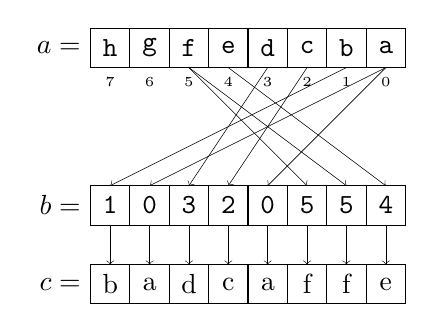
\begin{tikzpicture}
\node[below] at (3.75, 0.00) {\tiny0};
\node[below] at (3.25, 0.00) {\tiny1};
\node[below] at (2.75, 0.00) {\tiny2};
\node[below] at (2.25, 0.00) {\tiny3};
\node[below] at (1.75, 0.00) {\tiny4};
\node[below] at (1.25, 0.00) {\tiny5};
\node[below] at (0.75, 0.00) {\tiny6};
\node[below] at (0.25, 0.00) {\tiny7};
\draw[very thin,->] (1.750,0.000) -- (3.750,-1.500);
\draw[very thin,->] (3.750,-2.000) -- (3.750,-2.500);
\draw[very thin,->] (1.250,0.000) -- (3.250,-1.500);
\draw[very thin,->] (3.250,-2.000) -- (3.250,-2.500);
\draw[very thin,->] (1.250,0.000) -- (2.750,-1.500);
\draw[very thin,->] (2.750,-2.000) -- (2.750,-2.500);
\draw[very thin,->] (3.750,0.000) -- (2.250,-1.500);
\draw[very thin,->] (2.250,-2.000) -- (2.250,-2.500);
\draw[very thin,->] (2.750,0.000) -- (1.750,-1.500);
\draw[very thin,->] (1.750,-2.000) -- (1.750,-2.500);
\draw[very thin,->] (2.250,0.000) -- (1.250,-1.500);
\draw[very thin,->] (1.250,-2.000) -- (1.250,-2.500);
\draw[very thin,->] (3.750,0.000) -- (0.750,-1.500);
\draw[very thin,->] (0.750,-2.000) -- (0.750,-2.500);
\draw[very thin,->] (3.250,0.000) -- (0.250,-1.500);
\draw[very thin,->] (0.250,-2.000) -- (0.250,-2.500);
\node[anchor=east] at (0.000,0.250) {$a=$};
\node[anchor=east] at (0.000,-1.750) {$b=$};
\node[anchor=east] at (0.000,-2.750) {$c=$};
\draw [fill=white] (3.50, 0.00) rectangle (4.00, 0.50);
\node at (3.75, 0.25) {\texttt{a}};
\draw [fill=white] (3.00, 0.00) rectangle (3.50, 0.50);
\node at (3.25, 0.25) {\texttt{b}};
\draw [fill=white] (2.50, 0.00) rectangle (3.00, 0.50);
\node at (2.75, 0.25) {\texttt{c}};
\draw [fill=white] (2.00, 0.00) rectangle (2.50, 0.50);
\node at (2.25, 0.25) {\texttt{d}};
\draw [fill=white] (1.50, 0.00) rectangle (2.00, 0.50);
\node at (1.75, 0.25) {\texttt{e}};
\draw [fill=white] (1.00, 0.00) rectangle (1.50, 0.50);
\node at (1.25, 0.25) {\texttt{f}};
\draw [fill=white] (0.50, 0.00) rectangle (1.00, 0.50);
\node at (0.75, 0.25) {\texttt{g}};
\draw [fill=white] (0.00, 0.00) rectangle (0.50, 0.50);
\node at (0.25, 0.25) {\texttt{h}};
\draw [fill=white] (3.50, -2.00) rectangle (4.00, -1.50);
\node at (3.75, -1.75) {\texttt{4}};
\draw [fill=white] (3.00, -2.00) rectangle (3.50, -1.50);
\node at (3.25, -1.75) {\texttt{5}};
\draw [fill=white] (2.50, -2.00) rectangle (3.00, -1.50);
\node at (2.75, -1.75) {\texttt{5}};
\draw [fill=white] (2.00, -2.00) rectangle (2.50, -1.50);
\node at (2.25, -1.75) {\texttt{0}};
\draw [fill=white] (1.50, -2.00) rectangle (2.00, -1.50);
\node at (1.75, -1.75) {\texttt{2}};
\draw [fill=white] (1.00, -2.00) rectangle (1.50, -1.50);
\node at (1.25, -1.75) {\texttt{3}};
\draw [fill=white] (0.50, -2.00) rectangle (1.00, -1.50);
\node at (0.75, -1.75) {\texttt{0}};
\draw [fill=white] (0.00, -2.00) rectangle (0.50, -1.50);
\node at (0.25, -1.75) {\texttt{1}};
\draw [] (3.50, -3.00) rectangle (4.00, -2.50);
\node at (3.75, -2.75) {e};
\draw [] (3.00, -3.00) rectangle (3.50, -2.50);
\node at (3.25, -2.75) {f};
\draw [] (2.50, -3.00) rectangle (3.00, -2.50);
\node at (2.75, -2.75) {f};
\draw [] (2.00, -3.00) rectangle (2.50, -2.50);
\node at (2.25, -2.75) {a};
\draw [] (1.50, -3.00) rectangle (2.00, -2.50);
\node at (1.75, -2.75) {c};
\draw [] (1.00, -3.00) rectangle (1.50, -2.50);
\node at (1.25, -2.75) {d};
\draw [] (0.50, -3.00) rectangle (1.00, -2.50);
\node at (0.75, -2.75) {a};
\draw [] (0.00, -3.00) rectangle (0.50, -2.50);
\node at (0.25, -2.75) {b};
\end{tikzpicture}

    \end{center}
}

\frame{
    \frametitle{Example of shuffle --- reverse}

    Operation is $c = \textrm{shuffle}(a, b)$

    \begin{center}
        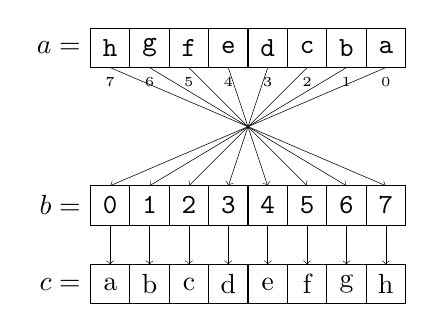
\begin{tikzpicture}
\node[below] at (3.75, 0.00) {\tiny0};
\node[below] at (3.25, 0.00) {\tiny1};
\node[below] at (2.75, 0.00) {\tiny2};
\node[below] at (2.25, 0.00) {\tiny3};
\node[below] at (1.75, 0.00) {\tiny4};
\node[below] at (1.25, 0.00) {\tiny5};
\node[below] at (0.75, 0.00) {\tiny6};
\node[below] at (0.25, 0.00) {\tiny7};
\draw[very thin,->] (0.250,0.000) -- (3.750,-1.500);
\draw[very thin,->] (3.750,-2.000) -- (3.750,-2.500);
\draw[very thin,->] (0.750,0.000) -- (3.250,-1.500);
\draw[very thin,->] (3.250,-2.000) -- (3.250,-2.500);
\draw[very thin,->] (1.250,0.000) -- (2.750,-1.500);
\draw[very thin,->] (2.750,-2.000) -- (2.750,-2.500);
\draw[very thin,->] (1.750,0.000) -- (2.250,-1.500);
\draw[very thin,->] (2.250,-2.000) -- (2.250,-2.500);
\draw[very thin,->] (2.250,0.000) -- (1.750,-1.500);
\draw[very thin,->] (1.750,-2.000) -- (1.750,-2.500);
\draw[very thin,->] (2.750,0.000) -- (1.250,-1.500);
\draw[very thin,->] (1.250,-2.000) -- (1.250,-2.500);
\draw[very thin,->] (3.250,0.000) -- (0.750,-1.500);
\draw[very thin,->] (0.750,-2.000) -- (0.750,-2.500);
\draw[very thin,->] (3.750,0.000) -- (0.250,-1.500);
\draw[very thin,->] (0.250,-2.000) -- (0.250,-2.500);
\node[anchor=east] at (0.000,0.250) {$a=$};
\node[anchor=east] at (0.000,-1.750) {$b=$};
\node[anchor=east] at (0.000,-2.750) {$c=$};
\draw [fill=white] (3.50, 0.00) rectangle (4.00, 0.50);
\node at (3.75, 0.25) {\texttt{a}};
\draw [fill=white] (3.00, 0.00) rectangle (3.50, 0.50);
\node at (3.25, 0.25) {\texttt{b}};
\draw [fill=white] (2.50, 0.00) rectangle (3.00, 0.50);
\node at (2.75, 0.25) {\texttt{c}};
\draw [fill=white] (2.00, 0.00) rectangle (2.50, 0.50);
\node at (2.25, 0.25) {\texttt{d}};
\draw [fill=white] (1.50, 0.00) rectangle (2.00, 0.50);
\node at (1.75, 0.25) {\texttt{e}};
\draw [fill=white] (1.00, 0.00) rectangle (1.50, 0.50);
\node at (1.25, 0.25) {\texttt{f}};
\draw [fill=white] (0.50, 0.00) rectangle (1.00, 0.50);
\node at (0.75, 0.25) {\texttt{g}};
\draw [fill=white] (0.00, 0.00) rectangle (0.50, 0.50);
\node at (0.25, 0.25) {\texttt{h}};
\draw [fill=white] (3.50, -2.00) rectangle (4.00, -1.50);
\node at (3.75, -1.75) {\texttt{7}};
\draw [fill=white] (3.00, -2.00) rectangle (3.50, -1.50);
\node at (3.25, -1.75) {\texttt{6}};
\draw [fill=white] (2.50, -2.00) rectangle (3.00, -1.50);
\node at (2.75, -1.75) {\texttt{5}};
\draw [fill=white] (2.00, -2.00) rectangle (2.50, -1.50);
\node at (2.25, -1.75) {\texttt{4}};
\draw [fill=white] (1.50, -2.00) rectangle (2.00, -1.50);
\node at (1.75, -1.75) {\texttt{3}};
\draw [fill=white] (1.00, -2.00) rectangle (1.50, -1.50);
\node at (1.25, -1.75) {\texttt{2}};
\draw [fill=white] (0.50, -2.00) rectangle (1.00, -1.50);
\node at (0.75, -1.75) {\texttt{1}};
\draw [fill=white] (0.00, -2.00) rectangle (0.50, -1.50);
\node at (0.25, -1.75) {\texttt{0}};
\draw [] (3.50, -3.00) rectangle (4.00, -2.50);
\node at (3.75, -2.75) {h};
\draw [] (3.00, -3.00) rectangle (3.50, -2.50);
\node at (3.25, -2.75) {g};
\draw [] (2.50, -3.00) rectangle (3.00, -2.50);
\node at (2.75, -2.75) {f};
\draw [] (2.00, -3.00) rectangle (2.50, -2.50);
\node at (2.25, -2.75) {e};
\draw [] (1.50, -3.00) rectangle (2.00, -2.50);
\node at (1.75, -2.75) {d};
\draw [] (1.00, -3.00) rectangle (1.50, -2.50);
\node at (1.25, -2.75) {c};
\draw [] (0.50, -3.00) rectangle (1.00, -2.50);
\node at (0.75, -2.75) {b};
\draw [] (0.00, -3.00) rectangle (0.50, -2.50);
\node at (0.25, -2.75) {a};
\end{tikzpicture}

    \end{center}
}

\frame{
    \frametitle{Example of shuffle --- broadcast}

    Operation is $c = \textrm{shuffle}(a, b)$

    \begin{center}
        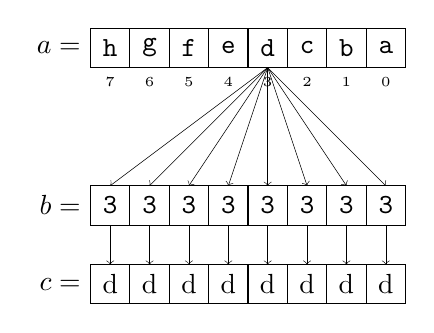
\begin{tikzpicture}
\node[below] at (3.75, 0.00) {\tiny0};
\node[below] at (3.25, 0.00) {\tiny1};
\node[below] at (2.75, 0.00) {\tiny2};
\node[below] at (2.25, 0.00) {\tiny3};
\node[below] at (1.75, 0.00) {\tiny4};
\node[below] at (1.25, 0.00) {\tiny5};
\node[below] at (0.75, 0.00) {\tiny6};
\node[below] at (0.25, 0.00) {\tiny7};
\draw[very thin,->] (2.250,0.000) -- (3.750,-1.500);
\draw[very thin,->] (3.750,-2.000) -- (3.750,-2.500);
\draw[very thin,->] (2.250,0.000) -- (3.250,-1.500);
\draw[very thin,->] (3.250,-2.000) -- (3.250,-2.500);
\draw[very thin,->] (2.250,0.000) -- (2.750,-1.500);
\draw[very thin,->] (2.750,-2.000) -- (2.750,-2.500);
\draw[very thin,->] (2.250,0.000) -- (2.250,-1.500);
\draw[very thin,->] (2.250,-2.000) -- (2.250,-2.500);
\draw[very thin,->] (2.250,0.000) -- (1.750,-1.500);
\draw[very thin,->] (1.750,-2.000) -- (1.750,-2.500);
\draw[very thin,->] (2.250,0.000) -- (1.250,-1.500);
\draw[very thin,->] (1.250,-2.000) -- (1.250,-2.500);
\draw[very thin,->] (2.250,0.000) -- (0.750,-1.500);
\draw[very thin,->] (0.750,-2.000) -- (0.750,-2.500);
\draw[very thin,->] (2.250,0.000) -- (0.250,-1.500);
\draw[very thin,->] (0.250,-2.000) -- (0.250,-2.500);
\node[anchor=east] at (0.000,0.250) {$a=$};
\node[anchor=east] at (0.000,-1.750) {$b=$};
\node[anchor=east] at (0.000,-2.750) {$c=$};
\draw [fill=white] (3.50, 0.00) rectangle (4.00, 0.50);
\node at (3.75, 0.25) {\texttt{a}};
\draw [fill=white] (3.00, 0.00) rectangle (3.50, 0.50);
\node at (3.25, 0.25) {\texttt{b}};
\draw [fill=white] (2.50, 0.00) rectangle (3.00, 0.50);
\node at (2.75, 0.25) {\texttt{c}};
\draw [fill=white] (2.00, 0.00) rectangle (2.50, 0.50);
\node at (2.25, 0.25) {\texttt{d}};
\draw [fill=white] (1.50, 0.00) rectangle (2.00, 0.50);
\node at (1.75, 0.25) {\texttt{e}};
\draw [fill=white] (1.00, 0.00) rectangle (1.50, 0.50);
\node at (1.25, 0.25) {\texttt{f}};
\draw [fill=white] (0.50, 0.00) rectangle (1.00, 0.50);
\node at (0.75, 0.25) {\texttt{g}};
\draw [fill=white] (0.00, 0.00) rectangle (0.50, 0.50);
\node at (0.25, 0.25) {\texttt{h}};
\draw [fill=white] (3.50, -2.00) rectangle (4.00, -1.50);
\node at (3.75, -1.75) {\texttt{3}};
\draw [fill=white] (3.00, -2.00) rectangle (3.50, -1.50);
\node at (3.25, -1.75) {\texttt{3}};
\draw [fill=white] (2.50, -2.00) rectangle (3.00, -1.50);
\node at (2.75, -1.75) {\texttt{3}};
\draw [fill=white] (2.00, -2.00) rectangle (2.50, -1.50);
\node at (2.25, -1.75) {\texttt{3}};
\draw [fill=white] (1.50, -2.00) rectangle (2.00, -1.50);
\node at (1.75, -1.75) {\texttt{3}};
\draw [fill=white] (1.00, -2.00) rectangle (1.50, -1.50);
\node at (1.25, -1.75) {\texttt{3}};
\draw [fill=white] (0.50, -2.00) rectangle (1.00, -1.50);
\node at (0.75, -1.75) {\texttt{3}};
\draw [fill=white] (0.00, -2.00) rectangle (0.50, -1.50);
\node at (0.25, -1.75) {\texttt{3}};
\draw [] (3.50, -3.00) rectangle (4.00, -2.50);
\node at (3.75, -2.75) {d};
\draw [] (3.00, -3.00) rectangle (3.50, -2.50);
\node at (3.25, -2.75) {d};
\draw [] (2.50, -3.00) rectangle (3.00, -2.50);
\node at (2.75, -2.75) {d};
\draw [] (2.00, -3.00) rectangle (2.50, -2.50);
\node at (2.25, -2.75) {d};
\draw [] (1.50, -3.00) rectangle (2.00, -2.50);
\node at (1.75, -2.75) {d};
\draw [] (1.00, -3.00) rectangle (1.50, -2.50);
\node at (1.25, -2.75) {d};
\draw [] (0.50, -3.00) rectangle (1.00, -2.50);
\node at (0.75, -2.75) {d};
\draw [] (0.00, -3.00) rectangle (0.50, -2.50);
\node at (0.25, -2.75) {d};
\end{tikzpicture}

    \end{center}
}

\frame{
    \frametitle{Example of blend}

    Operation is $c = s\ ?\ a : b$

    \begin{center}
        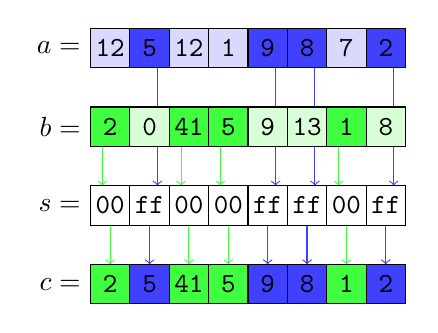
\begin{tikzpicture}
\draw[color=blue!75,->] (3.850,0.000) -- (3.850,-1.500);
\draw[color=blue!75,->] (3.750,-2.000) -- (3.750,-2.500);
\draw[color=green!75,->] (3.150,-1.000) -- (3.150,-1.500);
\draw[color=green!75,->] (3.250,-2.000) -- (3.250,-2.500);
\draw[color=blue!75,->] (2.850,0.000) -- (2.850,-1.500);
\draw[color=blue!75,->] (2.750,-2.000) -- (2.750,-2.500);
\draw[color=blue!75,->] (2.350,0.000) -- (2.350,-1.500);
\draw[color=blue!75,->] (2.250,-2.000) -- (2.250,-2.500);
\draw[color=green!75,->] (1.650,-1.000) -- (1.650,-1.500);
\draw[color=green!75,->] (1.750,-2.000) -- (1.750,-2.500);
\draw[color=green!75,->] (1.150,-1.000) -- (1.150,-1.500);
\draw[color=green!75,->] (1.250,-2.000) -- (1.250,-2.500);
\draw[color=blue!75,->] (0.850,0.000) -- (0.850,-1.500);
\draw[color=blue!75,->] (0.750,-2.000) -- (0.750,-2.500);
\draw[color=green!75,->] (0.150,-1.000) -- (0.150,-1.500);
\draw[color=green!75,->] (0.250,-2.000) -- (0.250,-2.500);
\node[anchor=east] at (0.000,0.250) {$a=$};
\node[anchor=east] at (0.000,-0.750) {$b=$};
\node[anchor=east] at (0.000,-1.750) {$s=$};
\node[anchor=east] at (0.000,-2.750) {$c=$};
\draw [fill=blue!75] (3.50, 0.00) rectangle (4.00, 0.50);
\node at (3.75, 0.25) {\texttt{2}};
\draw [fill=blue!15] (3.00, 0.00) rectangle (3.50, 0.50);
\node at (3.25, 0.25) {\texttt{7}};
\draw [fill=blue!75] (2.50, 0.00) rectangle (3.00, 0.50);
\node at (2.75, 0.25) {\texttt{8}};
\draw [fill=blue!75] (2.00, 0.00) rectangle (2.50, 0.50);
\node at (2.25, 0.25) {\texttt{9}};
\draw [fill=blue!15] (1.50, 0.00) rectangle (2.00, 0.50);
\node at (1.75, 0.25) {\texttt{1}};
\draw [fill=blue!15] (1.00, 0.00) rectangle (1.50, 0.50);
\node at (1.25, 0.25) {\texttt{12}};
\draw [fill=blue!75] (0.50, 0.00) rectangle (1.00, 0.50);
\node at (0.75, 0.25) {\texttt{5}};
\draw [fill=blue!15] (0.00, 0.00) rectangle (0.50, 0.50);
\node at (0.25, 0.25) {\texttt{12}};
\draw [fill=green!15] (3.50, -1.00) rectangle (4.00, -0.50);
\node at (3.75, -0.75) {\texttt{8}};
\draw [fill=green!75] (3.00, -1.00) rectangle (3.50, -0.50);
\node at (3.25, -0.75) {\texttt{1}};
\draw [fill=green!15] (2.50, -1.00) rectangle (3.00, -0.50);
\node at (2.75, -0.75) {\texttt{13}};
\draw [fill=green!15] (2.00, -1.00) rectangle (2.50, -0.50);
\node at (2.25, -0.75) {\texttt{9}};
\draw [fill=green!75] (1.50, -1.00) rectangle (2.00, -0.50);
\node at (1.75, -0.75) {\texttt{5}};
\draw [fill=green!75] (1.00, -1.00) rectangle (1.50, -0.50);
\node at (1.25, -0.75) {\texttt{41}};
\draw [fill=green!15] (0.50, -1.00) rectangle (1.00, -0.50);
\node at (0.75, -0.75) {\texttt{0}};
\draw [fill=green!75] (0.00, -1.00) rectangle (0.50, -0.50);
\node at (0.25, -0.75) {\texttt{2}};
\draw [fill=white] (3.50, -2.00) rectangle (4.00, -1.50);
\node at (3.75, -1.75) {\texttt{ff}};
\draw [fill=white] (3.00, -2.00) rectangle (3.50, -1.50);
\node at (3.25, -1.75) {\texttt{00}};
\draw [fill=white] (2.50, -2.00) rectangle (3.00, -1.50);
\node at (2.75, -1.75) {\texttt{ff}};
\draw [fill=white] (2.00, -2.00) rectangle (2.50, -1.50);
\node at (2.25, -1.75) {\texttt{ff}};
\draw [fill=white] (1.50, -2.00) rectangle (2.00, -1.50);
\node at (1.75, -1.75) {\texttt{00}};
\draw [fill=white] (1.00, -2.00) rectangle (1.50, -1.50);
\node at (1.25, -1.75) {\texttt{00}};
\draw [fill=white] (0.50, -2.00) rectangle (1.00, -1.50);
\node at (0.75, -1.75) {\texttt{ff}};
\draw [fill=white] (0.00, -2.00) rectangle (0.50, -1.50);
\node at (0.25, -1.75) {\texttt{00}};
\draw [fill=blue!75] (3.50, -3.00) rectangle (4.00, -2.50);
\node at (3.75, -2.75) {\texttt{2}};
\draw [fill=green!75] (3.00, -3.00) rectangle (3.50, -2.50);
\node at (3.25, -2.75) {\texttt{1}};
\draw [fill=blue!75] (2.50, -3.00) rectangle (3.00, -2.50);
\node at (2.75, -2.75) {\texttt{8}};
\draw [fill=blue!75] (2.00, -3.00) rectangle (2.50, -2.50);
\node at (2.25, -2.75) {\texttt{9}};
\draw [fill=green!75] (1.50, -3.00) rectangle (2.00, -2.50);
\node at (1.75, -2.75) {\texttt{5}};
\draw [fill=green!75] (1.00, -3.00) rectangle (1.50, -2.50);
\node at (1.25, -2.75) {\texttt{41}};
\draw [fill=blue!75] (0.50, -3.00) rectangle (1.00, -2.50);
\node at (0.75, -2.75) {\texttt{5}};
\draw [fill=green!75] (0.00, -3.00) rectangle (0.50, -2.50);
\node at (0.25, -2.75) {\texttt{2}};
\end{tikzpicture}

    \end{center}

    As a raw bit operations  $c = (s \mathop{\textrm{and}} a) \mathop{\textrm{or}} (\mathop{\textrm{not}} s \mathop{\textrm{and}} b)$
}

\frame{
    \frametitle{Integer saturated arithmetic}

    \begin{itemize}
        \pause
        \item A unique feature of SIMD
        \pause
        \item \ldots but something popular in the DSP world
        \pause
        \item Prevents from overflows during integer operations
        \pause
        \item \ldots saves min or max value for given type
        \pause
        \item \ldots 0 or 255 for 8-bit unsigned integers
        \pause
        \item Wrap-around (modulo) arithmetic:
        \pause
        \item \hspace{0.5cm} $(240 + 100) \mod 256 = 84$
        \pause
        \item Saturated arithmetics:
        \pause
        \item \hspace{0.5cm} $\min(240 + 100, 255) = \min(340, 255) = 255$
        \pause
        \item Saturated arithmetic is as fast as wrap-around one
    \end{itemize}
}

\frame{
    \frametitle{Saturated addition example --- increase image brightness}

    \newbox\original
    \setbox\original\hbox{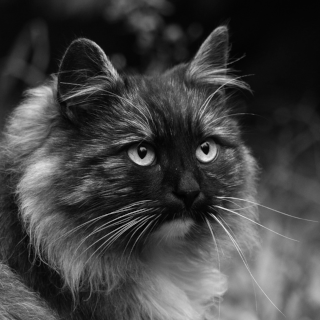
\includegraphics[scale=0.25]{cat_grayscale}}

    \newbox\addwrap
    \setbox\addwrap\hbox{\includegraphics[scale=0.25]{cat_add_wrap}}

    \newbox\addsat
    \setbox\addsat\hbox{\includegraphics[scale=0.25]{cat_add_sat}}

    \pause
    Wrap-around arithmetic

    \begin{center}
        \usebox\original
        \vbox to \ht\original {\vfill \hbox {\huge\ + 180 =\ }\vfill}
        \usebox\addwrap
    \end{center}

    \pause
    Saturated arithmetic

    \begin{center}
        \usebox\original
        \vbox to \ht\original {\vfill \hbox {\huge\ + 180 =\ }\vfill}
        \usebox\addsat
    \end{center}
}

\frame{
    \frametitle{SIMD instructions in real life}

    How about adding two vectors of arbitrary size?  ($c = a + b$)

    \pause
    \begin{adjustbox}{max width=10cm}
        \lstinputlisting[language=C++,numbers=left]{vector-add.cpp}
    \end{adjustbox}

    \vfill

    \pause
    Function \texttt{vector\_add} can rewritten (\emph{vectorized}) as:

    \vfill

    \begin{adjustbox}{max width=10cm}
    \lstinputlisting[language=C++,numbers=left]{vector-add-simd.cpp}
    \end{adjustbox}

    \vfill
}

\frame{
    \frametitle{Is it really better?}

    \begin{adjustbox}{max width=8cm}
    \lstinputlisting[language=C++,numbers=left]{vector-add-simd.cpp}
    \end{adjustbox}

    \vfill

    \begin{itemize}
        \pause
        \item Now it is more complicated, as there are \textbf{two loops}
        \pause
        \item We need to know how these magic \texttt{vector\_foo} functions
              work to reason about the code
        \pause
        \item The additional loop processes the \textbf{tail} of input --- it
              will execute just $0 \ldots 7$ iterations, but has to (re)implement
              whole logic of the main loop
        \pause
        \item What if we wanted to port it for another CPU, which is capable
              to process 16, 32 or 64 numbers?
    \end{itemize}
}

\frame{
    \frametitle{But SIMD is faster!}

    \pause
    More complex code pays off in peformance boost

    {\tiny Results gathered from several articles from my website}


    \begin{itemize}
        % http://0x80.pl/notesen/2016-01-17-sse-base64-decoding.html#experiments-update
        \pause
        \item base64 decoding: \hfill
              2 x faster

        % http://0x80.pl/articles/reverse-array-of-bytes.html
        \pause
        \item reverse table: \hfill
              3 x faster

        % http://0x80.pl/notesen/2018-10-24-sse-sumbytes.html
        \pause
        \item summing bytes: \hfill
              4 x faster

        % http://0x80.pl/notesen/2016-01-12-sse-base64-encoding.html
        \pause
        \item base64 encoding: \hfill
              4 x faster

        % http://0x80.pl/articles/sse-popcount.html
        \pause
        \item population count: \hfill
              5 x faster

        % http://0x80.pl/articles/sse-pix16to32bpp.html
        \pause
        \item pixel format conversions: \hfill
              5 x faster

        % http://0x80.pl/articles/sse4-alphaover.html
        \pause
        \item images mixing: \hfill
              7 x faster

        % http://0x80.pl/notesen/2018-05-13-avx512-jpeg-zigzag-transform.html
        \pause
        \item JPEG zig-zag transformation: \hfill
              7 x faster

        % http://0x80.pl/notesen/2018-04-11-simd-is-sorted.html
        \pause
        \item \texttt{std::is\_sorted}: \hfill
              8 x faster

        % http://0x80.pl/notesen/2018-10-03-simd-index-of-min.html
        \pause
        \item finding index of min element: \hfill
              14 x faster
    \end{itemize}
}

\frame{
    \frametitle{When does SIMD shine?}

    \begin{itemize}
        \pause
        \item SIMD fits well for arithmetic-insensitive problems
        \pause
        \item \ldots dead simple calculations
        \pause
        \item \ldots no \texttt{if} / \texttt{switch}
        \pause
        \item \ldots no data dependencies between iterations
        \pause
        \item SIMD requires regular data access
        \pause
        \item \ldots preferably sequential access
        \pause
        \item \ldots no pointers / computed indices
        \pause
        \item \ldots no calls to external functions
        \pause
        \item SIMD requires designed data structures to use full power
    \end{itemize}
}

\frame{
    \frametitle{More realistic example --- signal mixing}

    Following vector code mixes two signals (image, sound) using linear interpolation

    $$c = a \cdot p + b \cdot (1 - p), p \in [0, 1]$$

    \begin{adjustbox}{max width=11cm}
    \lstinputlisting[language=C++,numbers=left]{vector-lerp-simd.cpp}
    \end{adjustbox}
}

\frame{
    \frametitle{SIMD for programmers}

    \begin{itemize}
        \pause
        \item Currently no programming languages directly support SIMD data types
        \pause
        \item Exception is a C extension \textbf{ispc}
              (\href{https://ispc.github.io/}{ispc.github.io})
        \pause
        \item SIMD instructions are available for programmers as so called
              \textbf{intrinsic} functions (in our examples \texttt{vector\_foo})
        \pause
        \item Intrinsic functions are translated by compilers into a~predefined
              sequence of CPU instructions, often just one
        \pause
        \item There are attempts to hide multitude of SIMD flavours
              behind some generic API, may be worth to check out.
        \pause
        \item Compilers can \textbf{autovectorize} loops --- they do
              similar transformation as we did to \texttt{vector\_add}
        \pause
        \item Autovectorization is not as smart as human, but is decent
    \end{itemize}
}

\frame{
    \frametitle{Signal mixing in practise}

    This is actual C++ code for signal mixing which uses Intel intrinsics
    functions for AVX2 extension (full list on
    \href{https://software.intel.com/sites/landingpage/IntrinsicsGuide/}{Intrinsics Guide})

    \begin{adjustbox}{max width=10cm}
    \lstinputlisting[language=C++,numbers=left]{vector-lerp-avx2.cpp}
    \end{adjustbox}

    \pause
    It compiles! \texttt{gcc -mavx2 -c vector-lerp-avx2.cpp}
}

\frame{
    \frametitle{Takeaways}

    \begin{itemize}
        \pause
        \item SIMD instructions are ubiquitous
        \pause
        \item SIMD can give significant speedup
        \pause
        \item \ldots but doesn't make a program magically faster
        \pause
        \item SIMD instructions are quite hard to master by programmers
        \pause
        \item \ldots our mental model is different
        \pause
        \item \ldots training helps
        \pause
        \item Luckily compilers are getting better in autovectorization
        \pause
        \item More and more software libraries use SIMD instructions,
              we can benefit from it without changing our code
    \end{itemize}
}

\end{document}

\frame{
    \frametitle{}

    \begin{itemize}
        \pause
        \item
        \pause
        \item
        \pause
        \item
        \pause
        \item
        \pause
        \item
        \pause
        \item
        \pause
        \item
    \end{itemize}
}
